\documentclass[11pt]{article}

\usepackage[utf8]{inputenc}
\usepackage[margin=1in]{geometry}
\usepackage{hyperref}
\usepackage{graphicx}
\usepackage{booktabs}
\usepackage{amsmath}
\usepackage{amssymb}
\usepackage{xcolor}
\usepackage{natbib}
\usepackage{tikz}
\usetikzlibrary{arrows.meta, positioning, shapes.geometric}

\hypersetup{
  colorlinks=true,
  linkcolor=blue,
  citecolor=blue,
  urlcolor=blue
}

\title{Correlation-First Blame Propagation: Personalized PageRank and
Parameter-Free Change-Point Detection as Pre-LLM Graph Priors for
Root-Cause Analysis}

\author{Victor Robin\\ BlueRobin (independent homelab research)}

\date{June 2026}

\begin{document}

\maketitle

\begin{abstract}
This paper describes the deterministic, training-free pre-LLM scoring layer of
the BlueRobin Debug Agent, an advisory root-cause-analysis (RCA) system for a
self-hosted homelab operated under a hard $\approx$50~EUR/month budget. Before
any large-language-model (LLM) tokens are spent, the system seeds the agent's
hypothesis space with a ranked candidate list produced entirely by classical,
parameter-free graph and time-series statistics. The core is a four-stage
pipeline: (1)~an error-rate-weighted \emph{personalized PageRank} over the
runtime dependency graph that propagates ``blame'' from the alerting (symptom)
service to the dependencies it transitively calls; (2)~a Bayesian
repeat-offender history prior; (3)~a parameter-free Bayesian Online Change-Point
Detection (BOCPD) onset detector paired with a nonparametric, median-based
robust scorer in the style of BARO \citep{baro}; and (4)~a five-term
re-normalizing additive blend (\texttt{w\_topo=0.35}, \texttt{w\_tele=0.25},
\texttt{w\_hist=0.15}, \texttt{w\_chg=0.15}, \texttt{w\_baro=0.10}) that provably
collapses byte-for-byte to a topology/telemetry/history baseline when any lane is
absent. The design makes an explicit, repeatedly enforced architectural choice:
it uses \emph{correlation and change-point} signals only and rejects causal
discovery (PC/FCI/Granger/learned causal graphs), a decision validated against
two independent re-evaluations of the RCA literature
\citep{rcaeval,zhang2024causal} and policed by a CI reflection scan over the
scoring assembly. We report results on a self-seeded nine-incident benchmark with
the explicit caveat---shared by the authors---that it is an oversimplified
benchmark and that the reported MTTR figures are sub-second replay-clock proxies,
not production mean-time-to-resolution.
\end{abstract}

\section{Introduction}

Modern microservice RCA increasingly reaches for an LLM agent: a ReAct-style
\citep{react} loop that calls observability tools, reads traces and logs, and
narrates a hypothesis. The honest published ceiling for \emph{autonomous} LLM RCA
is low---the best agent on OpenRCA \citep{openrca} reaches roughly 11.3\%
exact-match, and the best frontier model on ITBench-AA \citep{itbenchaa} roughly
47\% precision-at-full-recall. LLM-only RCA is also structurally fragile: it lacks
grounding in system topology, it hallucinates plausible-but-wrong causes,
and---per the MAST failure taxonomy \citep{mast}---its dominant failure modes are
\emph{incorrect self-verification} and \emph{premature termination}. An agent
dropped cold into a tool loop wastes its turn budget rediscovering the obvious
shape of the system on every incident.

The pre-LLM scoring layer described here addresses the \emph{cold-start} problem
directly. Rather than asking the model to find the needle from scratch, the system
computes a ranked candidate list deterministically and injects it into the prompt
as ``prioritised leads to confirm, not conclusions.'' The leads come from cheap,
well-understood statistics that independent benchmarks show \emph{beat} the
expensive causal-discovery machinery on real data. The LLM's job is then
verification and narration, not blind search.

The contributions of this paper are:

\begin{itemize}
  \item \textbf{An error-weighted personalized PageRank ``blame propagation''
    pre-ranker} (\texttt{PageRank.cs}, \texttt{RootCauseRanker.cs}) that seeds the
    teleport vector at the symptom service and amplifies blame flow along
    high-error dependency edges---a power-iteration computation with no external
    dependency, fully deterministic, computed in microseconds on a
    homelab-sized graph.
  \item \textbf{A parameter-free BOCPD onset detector plus a nonparametric robust
    scorer} (\texttt{BaroAnomalyScorer.cs}) that reproduces the BARO recipe in
    dependency-free C\#: no hazard knob, no training, no GPU, total on degenerate
    input.
  \item \textbf{A five-term re-normalizing additive blend}
    (\texttt{BaroBlendScorer.cs}) with a \emph{provable fail-open collapse}: when
    the change lane and/or BARO lane are absent, the blend reduces byte-for-byte
    to a two- or three-term baseline, so the ranker degrades gracefully rather
    than failing closed.
  \item \textbf{An explicit, CI-enforced rejection of causal discovery.} The
    scoring assembly carries no PC/FCI/Granger/causal-graph code, and a reflection
    scan (TS-57) fails the build if a causal symbol appears. We justify this
    against the literature rather than asserting it.
  \item \textbf{A budget-first systems posture.} The entire layer runs inside an
    already-deployed 2~GiB FalkorDB instance with zero new always-on workload,
    consistent with the platform's $\approx$50~EUR/month ceiling.
\end{itemize}

This is a systems / experience report, not an empirical breakthrough. The layer
is advisory by design---a human always merges---and the evaluation is
deliberately modest.

\section{Related Work}

\paragraph{Classical and statistical RCA.}
Spectrum-and-random-walk methods rank suspect services by propagating anomaly
mass over a dependency graph. MicroRank \citep{microrank} combines spectrum
analysis with PageRank-style blame propagation; TraceRCA \citep{tracerca} mines
suspicious sets from anomalous traces and ranks by conditional probability. BARO
\citep{baro} detects the failure \emph{onset} with multivariate BOCPD and then
ranks with a nonparametric RobustScorer; it is parameter-free, training-free, and
runs in roughly 0.01~s. Our pre-LLM layer sits squarely in this family:
error-weighted personalized PageRank for propagation, plus a hand-rolled BARO core
for onset and robust ranking.

\paragraph{Causal RCA, and why we decline it.}
A parallel line of work learns a causal graph and infers the root from it: CIRCA
\citep{circa} frames a fault as an intervention and applies a regression-based
hypothesis test; RCD \citep{rcd} does localized causal discovery with a $\psi$-PC
variant; RUN \citep{run} combines neural Granger causality with personalized
PageRank. The decisive evidence against adopting causal \emph{discovery} in our
setting comes from two independent re-evaluations. RCAEval \citep{rcaeval} re-runs
15 baselines across 735 cases and finds correlation methods (BARO Avg@5 0.80,
TraceRCA 0.77) decisively beating causal ones (CIRCA 0.46, MicroCause 0.20, RCD
0.13). ``Root Cause Analysis with LLMs\ldots How Far Are We from Causal
Inference?'' \citep{zhang2024causal} finds PC/FCI/Granger full-graph methods are
``no better or only slightly better than random,'' require the \emph{exact}
failure time (a 60~s error degrades them significantly), and blow up
computationally (PC+KCI exceeding an hour per case at ten nodes versus BARO's
$\approx$0.01~s). The defensible causal \emph{idea}---``fault as
intervention''---survives in our change-correlation term; the
\emph{graph-learning step} is the weak, expensive link we drop.

\paragraph{Anomaly detection.}
TSB-AD \citep{tsbad} benchmarks 40 algorithms over 1{,}070 series and concludes
that ``simpler architectures and statistical methods often yield better
performance''; foundation models neither win nor pay for their 10--50$\times$
slowdown. This is the empirical warrant for a median-based, distribution-free
robust scorer over a learned detector.

\paragraph{Benchmarks.}
OpenRCA \citep{openrca}, AIOpsLab \citep{aiopslab}, ITBench \citep{itbench} and
RCAEval \citep{rcaeval} supply the metric vocabulary (AC@k, Avg@k, MRR,
MTTD/MTTR/TTM) we adopt internally. RCAEval's AC@k/Avg@k/MRR is the closest
analogue to our own scorecard. A standing caveat \citep{rethinkrca} warns that
current RCA benchmarks are oversimplified and overstate real capability---a caveat
we apply to our own nine-incident set in Section~\ref{sec:limitations}.

\section{Method / Architecture}
\label{sec:method}

The pre-LLM layer transforms an incoming alert into a ranked list of candidate
root causes using only deterministic statistics. Figure~\ref{fig:pipeline} shows
where it sits.

\begin{figure}[ht]
\centering
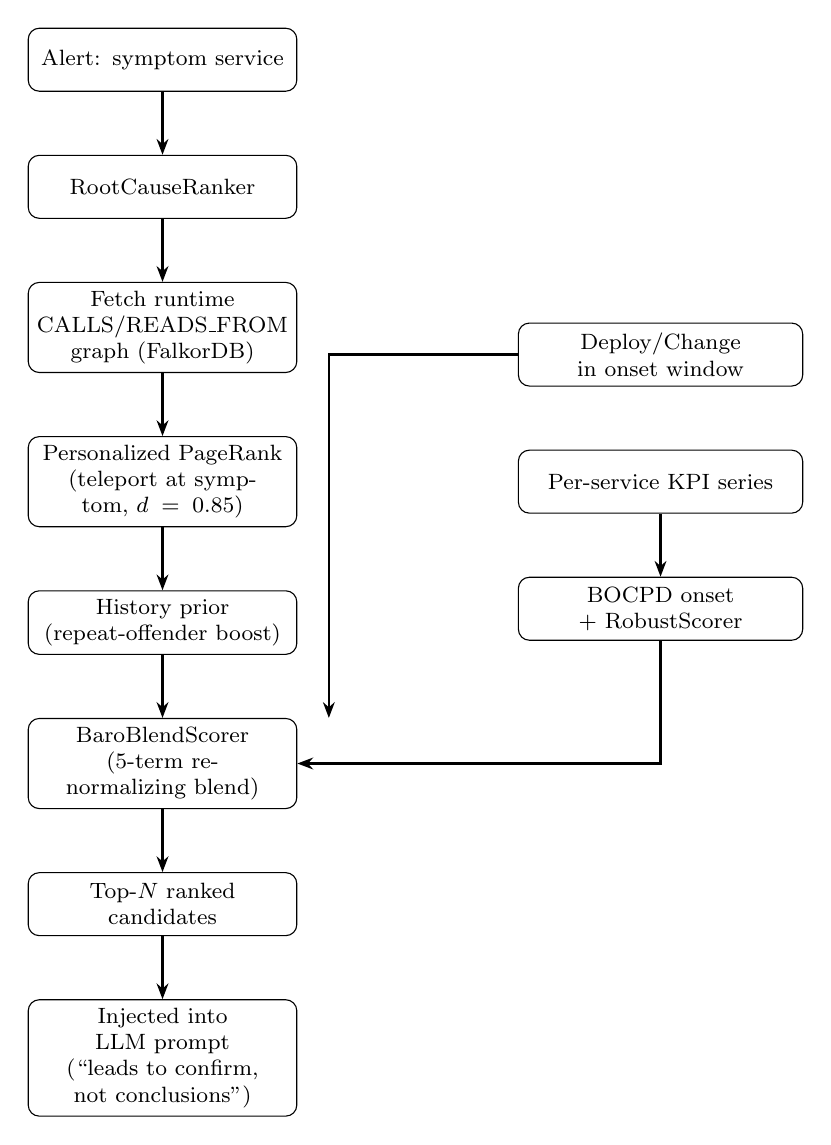
\begin{tikzpicture}[
  node distance=8mm and 12mm,
  box/.style={draw, rounded corners, align=center, font=\footnotesize,
    minimum height=8mm, inner sep=3pt, text width=32mm},
  arr/.style={-{Stealth[length=2mm]}, thick}
]
\node[box] (alert) {Alert: symptom service};
\node[box, below=of alert] (ranker) {RootCauseRanker};
\node[box, below=of ranker] (fetch) {Fetch runtime CALLS/READS\_FROM graph (FalkorDB)};
\node[box, below=of fetch] (ppr) {Personalized PageRank\\(teleport at symptom, $d=0.85$)};
\node[box, below=of ppr] (hist) {History prior\\(repeat-offender boost)};
\node[box, below=of hist] (blend) {BaroBlendScorer\\(5-term re-normalizing blend)};
\node[box, below=of blend] (topn) {Top-$N$ ranked candidates};
\node[box, below=of topn] (inject) {Injected into LLM prompt\\(``leads to confirm, not conclusions'')};

\node[box, right=28mm of ppr, text width=34mm] (kpi) {Per-service KPI series};
\node[box, below=of kpi, text width=34mm] (bocpd) {BOCPD onset + RobustScorer};
\node[box, above=of kpi, text width=34mm] (chg) {Deploy/Change in onset window};

\draw[arr] (alert) -- (ranker);
\draw[arr] (ranker) -- (fetch);
\draw[arr] (fetch) -- (ppr);
\draw[arr] (ppr) -- (hist);
\draw[arr] (hist) -- (blend);
\draw[arr] (blend) -- (topn);
\draw[arr] (topn) -- (inject);
\draw[arr] (kpi) -- (bocpd);
\draw[arr] (bocpd.south) |- (blend.east);
\draw[arr] (chg.west) -| ([xshift=4mm]blend.north east) ;
\end{tikzpicture}
\caption{The deterministic pre-LLM scoring pipeline. Every box is pure,
training-free, and runs before a single LLM token is spent.}
\label{fig:pipeline}
\end{figure}

\subsection{Personalized PageRank blame propagation}

The substrate is the runtime dependency graph:
\texttt{Service-[:CALLS|READS\_FROM]->Service} edges in the persistent
\texttt{bluerobin\_stack} FalkorDB graph, each carrying a measured
\texttt{error\_rate} from Tempo service-graph metrics.
\texttt{RootCauseRanker.RankAsync} (per \textbf{FEAT-027 / FR-SG-6}, the RCA query
API requirement) fetches the \emph{whole} runtime graph---it is small, tens of
edges on a homelab---with a single parameterless Cypher template, never
caller-interpolated (\textbf{SEC-SG-4}, parameterized Cypher only):

\begin{verbatim}
MATCH (a:Service)-[e:CALLS|READS_FROM]->(b:Service)
RETURN a.name, b.name, coalesce(e.error_rate, 0.0)
\end{verbatim}

Each directed edge is weighted
\begin{equation}
w(\text{from} \to \text{to}) = \text{BaseEdgeWeight}(0.1) + \text{error\_rate}.
\end{equation}
The base weight keeps the graph connected so blame can flow at all; the additive
\texttt{error\_rate} term amplifies flow toward failing dependencies. The ranker
then runs weighted \emph{personalized} PageRank (\texttt{PageRank.Run}), where the
personalization (teleport) vector is a point mass at the symptom service:

\begin{verbatim}
teleport   = { [symptomService] = 1.0 }   // all other nodes 0
damping    = 0.85
iterations = 50   // fixed -> deterministic, no tolerance nondeterminism
\end{verbatim}

Power iteration is initialized at the teleport distribution. At every step, mass
is mixed $(1-d)$ toward the teleport vector and $d$ along row-normalized
out-edges; dangling nodes (no usable out-edge) redistribute their mass through the
teleport vector. Because all blame re-injects at the symptom, score concentrates
on the dependencies the symptom transitively calls, weighted by how error-prone
those paths are. This is ``blame propagation'': the symptom is innocent of
\emph{being} the cause but is the seed from which suspicion flows downstream. The
implementation is pure and dependency-free, returns a distribution summing to
$\approx 1$, and is fully unit-tested. Per-node anomaly teleport (seeding mass at
\emph{every} anomalous service, not just the symptom) is noted in the code as a
deliberate future refinement; today the teleport is symptom-only.

\subsection{Bayesian repeat-offender history prior}
\label{sec:history}

PageRank scores for a candidate $c$ are folded with a multiplicative history
prior:
\begin{equation}
\text{score}'(c) = \text{score}(c) \cdot
\bigl(1 + \text{HistoryInfluence}(0.5) \cdot \text{prior}(c)\bigr),
\end{equation}
where $\text{prior}(c) \in [0,1]$ is a Bayesian repeat-offender estimate drawn
from the graph's RCA write-back history (\texttt{ROOT\_CAUSED\_BY} edges from past
validated incidents). A service that has been the validated root cause before is,
all else equal, a more credible candidate---a cheap Bayesian shrinkage toward
known offenders, capped at a 1.5$\times$ boost so history can never dominate live
error signal.

\subsection{Parameter-free BOCPD onset detection and the robust scorer}
\label{sec:bocpd}

The change-point lane (\texttt{BaroAnomalyScorer.cs}, per \textbf{FR-SG-30} and
\textbf{ADR-037 D5}) reproduces BARO in dependency-free C\#. It has three pieces.

\paragraph{\texttt{BocpdChangePoint.DetectOnset}.}
A parameter-free retrospective change-point detector over a single KPI series. It
sweeps every candidate boundary $k$ and chooses the one that maximizes the
two-segment Gaussian log-likelihood gain over the no-change (single-segment)
model, each segment scored under its own MLE mean and variance (the offline
reduction of a Normal--Gamma conjugate posterior). Crucially, \emph{no hazard or
threshold knob is passed in}: the significance test is a BIC-style penalty derived
from series length,
\begin{equation}
\text{onset} = \operatorname*{arg\,max}_{k}
\bigl[\, \mathrm{LL}(0,k) + \mathrm{LL}(k,n) - \mathrm{LL}(0,n) \,\bigr]
\quad \text{if gain} > \log(n), \;\text{else null},
\end{equation}
so a flat or stationary series yields \emph{no} onset---the fail-open sentinel
that prevents fabricating a change-point where none exists. A variance floor keeps
a perfect step finite. A minimum segment length of~3 guarantees each side has a
defined mean and variance.

\paragraph{\texttt{RobustScorer}.}
The nonparametric BARO scorer: the \emph{robust relative magnitude} of the
post-onset level shift, computed median-based and scale-free across heterogeneous
KPIs, with \textbf{no Gaussian/z-score assumption}. Bounded to $[0,1]$; exactly~0
when there is no onset or no shift.

\paragraph{\texttt{BaroAnomalyScorer}.}
The fa\c{c}ade the ranker consumes. Given a service's three Tempo service-graph
KPI series (\texttt{ServiceKpiSeries}: call-rate, error-ratio, p95-latency), it
returns the maximum robust shift across those KPIs as a bounded \texttt{baro}
sub-score (multivariate by max-pooling; $0 \Rightarrow$ no boost).

The whole core is pure, dependency-free, and total on empty/short input,
mirroring the existing \texttt{AnomalyStatistics} discipline.

\subsection{The five-term re-normalizing additive blend}
\label{sec:blend}

\texttt{BaroBlendScorer} (per \textbf{FR-SG-30}, \textbf{NFR-SG-2}, \textbf{ADR-037
\S T5}) fuses five deterministic sub-scores into one ranking score. The blend
evolved across increments; the canonical five-term form and its weights are given
in Table~\ref{tab:blend}.

\begin{table}[ht]
\centering
\caption{The canonical five-term blend.}
\label{tab:blend}
\begin{tabular}{llp{8cm}}
\toprule
Term & Weight & Source signal \\
\midrule
\texttt{topo} & \textbf{0.35} & topology criticality of the candidate service \\
\texttt{tele} & \textbf{0.25} & telemetry: measured error rate on the dependency edge (halved if the edge is \texttt{stale}) \\
\texttt{hist} & \textbf{0.15} & repeat-offender history prior (\S\ref{sec:history}) \\
\texttt{chg}  & \textbf{0.15} & onset-window change recency (Deploy/Change near the onset) \\
\texttt{baro} & \textbf{0.10} & BARO robust change-point sub-score (\S\ref{sec:bocpd}) \\
\bottomrule
\end{tabular}
\end{table}

The weights sum to 1.0. The change term $\text{chg}(c)$ is the maximum over
in-window Deploy/Change events of a recency ramp $1 - ((T - t_s)/W)$ over a
half-open onset window $[T - W, T]$ with $W = 1800$~s---privileging the deploy or
commit nearest the failure onset, the single strongest signal in the SRE
literature (Google's ``$\approx$70\% of outages are change-induced''
\citep{sre}).

The \textbf{fail-open collapse} is the load-bearing guarantee
(\textbf{NFR-SG-2}). When a lane's signal is absent---no Deploy/Change in window,
or a KPI series too short for BOCPD---the blend \emph{re-normalizes over the
present terms only} rather than penalizing the candidate with a zero. Concretely:

\begin{itemize}
  \item All five present $\to$ $0.35/0.25/0.15/0.15/0.10$.
  \item BARO absent, change present $\to$ the four-term blend $0.40/0.30/0.15/0.15$.
  \item Change and BARO both absent $\to$ the three-term baseline $0.50/0.35/0.15$
    (topo/tele/hist).
\end{itemize}

Each collapse is \emph{byte-for-byte identical} to the earlier-increment scorer it
reduces to---the four-term \texttt{OnsetWindowChangeScorer} delegates to the
three-term \texttt{RootCauseScorer} when the change lane is empty, and the
five-term \texttt{BaroBlendScorer} delegates to the four-term form when BARO is
empty. This is what lets the layer ship a richer ranker without risking a
regression: with the new lanes off, the output is provably the old output. Ties
break deterministically (score descending, then \texttt{NodeId} ascending)---a fix
for an early flaky AC@1 caused by FalkorDB returning rows in nondeterministic
order.

\subsection{The deliberate rejection of causal discovery}
\label{sec:nocausal}

The scoring assembly is annotated and tested as ``\,\emph{correlation +
change-point only---explicitly NO causal discovery (PC/FCI/Granger/causal-graph)}.''
This is not an omission; it is an enforced invariant. A reflection scan (TS-57)
runs over the analysis assembly in CI and fails the build if any causal-discovery
symbol is present. The justification is the Section~2 evidence: on independent
benchmarks, correlation and change-point beat learned causal graphs, while causal
discovery demands exact fault timing and prohibitive compute. The
``fault-as-intervention'' framing we \emph{do} keep---but it lives entirely in the
change-correlation term (a deploy in the onset window \emph{is} the intervention),
not in any structure-learning step.

\section{Implementation}

The layer is C\# (.NET~10), part of the Debug Agent service (FEAT-008 /
FEAT-027). Key types are listed in Table~\ref{tab:components}.

\begin{table}[ht]
\centering
\caption{Implementation components.}
\label{tab:components}
\begin{tabular}{lll}
\toprule
Component & File & Role \\
\midrule
\texttt{PageRank} & \texttt{Analysis/PageRank.cs} & pure weighted personalized PageRank (power iteration) \\
\texttt{RootCauseRanker} & \texttt{Analysis/RootCauseRanker.cs} & fetches the runtime graph, builds edge weights, runs PageRank + history prior \\
\texttt{BocpdChangePoint} & \texttt{Analysis/BaroAnomalyScorer.cs} & parameter-free BOCPD onset detection \\
\texttt{RobustScorer} / \texttt{BaroAnomalyScorer} & \texttt{Analysis/BaroAnomalyScorer.cs} & nonparametric robust shift magnitude $\to [0,1]$ \\
\texttt{OnsetWindowChangeScorer} & \texttt{StackGraph/OnsetWindowChangeScorer.cs} & four-term blend ($0.40/0.30/0.15/0.15$) \\
\texttt{BaroBlendScorer} & \texttt{StackGraph/BaroBlendScorer.cs} & five-term blend ($0.35/0.25/0.15/0.15/0.10$) \\
\bottomrule
\end{tabular}
\end{table}

\paragraph{Graph store.}
The runtime dependency graph lives in the existing FalkorDB instance
(\texttt{falkordb/falkordb:v4.4.1}, Redis wire protocol on port 6379, 2~GiB memory
limit) as a second graph key \texttt{bluerobin\_stack}, queried with parameterized
OpenCypher via \texttt{GRAPH.QUERY}. No second time-series database and no new
always-on workload is introduced; the \texttt{bluerobin} node is memory-saturated,
which is the binding constraint behind reusing the deployed FalkorDB rather than
standing up a dedicated graph engine.

\paragraph{Telemetry source.}
Edge \texttt{error\_rate} and the per-service KPI series come from Tempo's
metrics-generator service graphs (\texttt{traces\_service\_graph\_request\_*})---the
dependency graph and the RED signals are read from the same observability plane the
cluster already runs. Change/Deploy nodes are ingested from Flux reconciliations
and Git commits.

\paragraph{Cost.}
The entire pre-LLM layer consumes \emph{zero} LLM tokens: PageRank, BOCPD, the
robust scorer, and the blend are all CPU-only arithmetic over a tens-of-edges
graph and short KPI windows, completing in well under a millisecond. This is what
makes a graph-grounded RCA stack viable under the platform's hard ceiling---Hetzner
worker $\approx$ EUR~17.5/mo, Cloudflare R2/Tunnel free tier, and an LLM budget
capped at EUR~20/mo (COST-7), for $\approx$50~EUR/month total. The expensive
alternative---GraphRAG-style community indexing at roughly \$20--40 per 1M tokens,
or causal discovery at $>$1~hr/case---is explicitly out of budget. Spending the LLM
budget only on \emph{verifying} a deterministically-computed shortlist is the core
FinOps move.

The error-weighted personalized-PageRank seed is abridged as:
\begin{verbatim}
// RootCauseRanker.RankAsync -- error-weighted personalized PageRank seed
var weight = BaseEdgeWeight + (err > 0 ? err : 0);        // 0.1 + error_rate
var scores = PageRank.Run(
    nodes, outEdges,
    teleport: new Dictionary<string, double> { [symptomService] = 1.0 },
    damping: 0.85, iterations: 50);
// fold the repeat-offender prior: score * (1 + 0.5 * prior[node])
\end{verbatim}

The ranker is advisory and best-effort by contract (\textbf{NFR-SG-2}): an empty,
stale, or unreachable graph yields no candidates and never throws---the agent then
proceeds on its cold tool-floor. This fail-open posture is the same one the
blend's re-normalization enforces at the scoring level: every degradation path
returns a valid (possibly empty) ranking rather than an error.

\section{Evaluation}
\label{sec:eval}

The pre-LLM ranker is exercised by a deterministic offline replay harness
(\texttt{RcaEvalHarness}, per \textbf{FR-SG-23} / \textbf{ADR-036}) that replays a
labelled ground-truth incident set through the \emph{real} ranking path over a
seeded FalkorDB and emits an AC@1 + MTTR scorecard. The set is \textbf{nine
self-seeded labelled incidents} spanning three fault classes (auth/login,
data/datastore, deploy/config), drawn from existing synthetic faults---no
ChaosMesh---so the set is not trivially gameable.

The harness has two arms. The \textbf{scorer-only} arm plants the labelled cause
as an unambiguous top-1, so its AC@1 $= 1.0$ \emph{by construction}---a regression
sentinel, not an accuracy measure. The honest arm is \texttt{ReplayLivePathAsync},
the live-path arm, which derives onset from the alert and \textbf{injects
distractor candidates} (a deliberate topology trap: distractor criticality 0.95
\emph{above} the true cause's 0.9, distractor error-rate 0.55) so that AC@1
$< 1.0$ is achievable. Results are shown in Table~\ref{tab:scorecard}.

\begin{table}[ht]
\centering
\caption{Replay-harness scorecards on the nine-incident self-seeded set. MTTR is a
sub-second replay-clock proxy, not production mean-time-to-resolution.}
\label{tab:scorecard}
\begin{tabular}{lccccc}
\toprule
Arm & AC@1 & Avg@k & MRR & MTTR (s, replay-clock) & Incidents \\
\midrule
Scorer-only baseline (1.0 by construction) & 1.0 & 1.0 & 1.0 & 0.0017 & 9 \\
\textbf{Live-path baseline (distractors injected)} & \textbf{1.0} & 1.0 & 1.0 & 0.0032 & 9 \\
\bottomrule
\end{tabular}
\end{table}

On the nine-incident set, the ranker localizes the labelled root cause at top-1 in
all nine incidents \emph{even with distractors injected}. Avg@k and MRR reduce to
AC@1 here because each incident carries a single labelled cause scored at top-1
(per ADR-036 D1; extended when multi-candidate labels land). The per-commit merge
gate fails any candidate that drops AC@1 below 0.98 or inflates MTTR by more than
30~s (\texttt{GateTolerance(AcAt1Drop: 0.02, MttrSecondsIncrease: 30.0)}).

\paragraph{Ablations.}
Because the five-term blend collapses byte-for-byte when lanes are disabled, the
harness runs \emph{shadow-vs-active} ablations: with the BARO/change lanes in
shadow mode the scorecard is identical to the baseline (the ``feature off''
control), and the two change-induced incidents (GT-03 bad-deploy, GT-07
bad-commit) must keep AC@1 $= 1.0$ in every active-mode run---a guard that the new
lanes never \emph{suppress} a true positive they should have surfaced. There is no
graph-vs-no-graph ablation as a graded metric: the graph is the substrate of the
entire RCA path, and ``no graph'' surfaces only as the three-term fail-open floor.

\section{Limitations \& Threats to Validity}
\label{sec:limitations}

We state these plainly; the authors themselves call the benchmark oversimplified.

\begin{itemize}
  \item \textbf{The benchmark is small and self-seeded.} Nine incidents, three
    fault classes, labelled by the same authors who built the system. AC@1 $= 1.0$
    on this set is \emph{not} evidence of production accuracy. It is a regression
    sentinel and a sanity check, nothing more. External yardsticks (OpenRCA
    $\approx$11\%, ITBench-AA $\approx$47\%) are referenced as context, never as
    something this set is comparable to.
  \item \textbf{MTTR is a replay-clock proxy.} The reported sub-second MTTR figures
    are the wall-clock around an in-process replay, not time-to-resolution of a
    real incident. Production MTTD/MTTA/MTTR are computed separately from live
    lifecycle data (SLO-15/SLO-16), but no measured production value is claimed
    here.
  \item \textbf{The distractor trap is hand-designed.} The live-path arm's
    distractors are deliberately adversarial on topology but were authored by us; a
    different distractor distribution could lower AC@1. We make no claim that the
    trap is representative of real misleading topology.
  \item \textbf{Symptom-only teleport.} PageRank seeds blame solely at the alerting
    service. Multi-symptom incidents, where several services are independently
    anomalous, are not yet modeled by per-node anomaly teleport (a noted future
    refinement). Single-root-cause is an assumption baked into the current scorer.
  \item \textbf{Correlation is not causation---by design.} We deliberately do
    \emph{not} attempt causal discovery, so the ranker can be fooled by a
    confounded correlation (e.g.\ a shared upstream that fails two services at
    once). The change-correlation term mitigates but does not eliminate this; the
    human-in-the-loop merge is the backstop.
  \item \textbf{Advisory only.} Nothing auto-remediates. Every output is a lead for
    a human reviewer. This matches the state of the art for autonomous RCA rather
    than conceding a limitation---but it does mean the layer's value is measured by
    how well it \emph{focuses} a human, which this benchmark does not capture.
\end{itemize}

\section{Conclusion}

The pre-LLM scoring layer demonstrates that a large fraction of the RCA problem
can be handled \emph{before} the LLM ever runs, using deterministic, training-free
statistics that the independent literature shows outperform expensive causal
discovery. Error-weighted personalized PageRank propagates blame from symptom to
suspect; a parameter-free BOCPD onset detector and a nonparametric robust scorer
reproduce BARO with no training and no GPU; and a five-term re-normalizing blend
fuses these with a provable fail-open collapse to a baseline. The whole layer runs
in microseconds inside an already-deployed FalkorDB, consuming no LLM tokens, which
is precisely what makes a graph-grounded agentic RCA stack feasible at
$\approx$50~EUR/month. The headline is not an accuracy number---our benchmark is
too small and too friendly for that---but an architecture: spend deterministic
compute to build a shortlist, spend scarce LLM tokens only to verify it, and
refuse, on the evidence, to learn a causal graph.

\bibliographystyle{plainnat}
\bibliography{references}

\end{document}
